\documentclass[a4paper,10pt]{article}

\usepackage[english]{babel}
\usepackage[T1]{fontenc}
\usepackage[ansinew]{inputenc}

\usepackage{lmodern}	% font definition
\usepackage{amsmath}	% math fonts
\usepackage{amsthm}
\usepackage{amsfonts}
\usepackage{amssymb}
\usepackage{mathrsfs}
\usepackage{graphicx}

\usepackage{tikz}
\usepackage{ifthen}

%%%<
\usepackage{verbatim}
\usepackage[active,tightpage]{preview}
\PreviewEnvironment{tikzpicture}
\setlength\PreviewBorder{5pt}%
%%%>


\usetikzlibrary{decorations.pathmorphing} % noisy shapes
\usetikzlibrary{fit}					% fitting shapes to coordinates
\usetikzlibrary{backgrounds}	% drawing the background after the foreground
\usetikzlibrary{arrows.meta}
\usetikzlibrary{calc,positioning,shapes.geometric} 

\begin{document}

\tikzstyle{places}=[circle,draw=blue!50,fill=blue!20,thick,minimum
   size=5mm]
\tikzstyle{placef}=[rectangle,draw=black!50,fill=green!20,thick,minimum
   size=5mm,inner sep=0.1cm,rounded corners=2mm,opacity=0.99]
\tikzstyle{placef1}=[rectangle,draw=black!50,fill=green!20,thick,minimum
   size=5mm,inner sep=0.05cm,rounded corners=1mm,opacity=0.99]
\tikzstyle{placef2}=[rectangle,draw=black!50,fill=blue!20,thick,minimum
   size=5mm,inner sep=0.05cm,rounded corners=1mm,opacity=0.99]
\tikzstyle{placef3}=[rectangle,draw=black!50,fill=red!20,thick,minimum
   size=5mm,inner sep=0.05cm,rounded corners=1mm,opacity=0.99]
\tikzstyle{database}=[cylinder, cylinder uses custom fill,
   cylinder body fill=red!20,cylinder end fill=red!20,
   shape border rotate=90,aspect=0.15,draw] 
\tikzstyle{placeo1}=[circle,draw=black!50,fill=red!30,thick,minimum
   size=4mm]
\tikzstyle{placeo2}=[rectangle,draw=black!50,fill=blue!20,thick,minimum
   size=4mm]
\tikzstyle{placeo3}=[circle,draw=black!50,fill=green!30,thick,minimum
   size=4mm]
\tikzstyle{placeo4}=[circle,draw=black!50,fill=cyan!30,thick,minimum
   size=4mm]
\tikzstyle{placet}=[circle,draw=black!90,fill=blue!30,thick,
  minimum size=5mm,
  decorate,decoration={random steps,segment length=2pt,
                                 amplitude=1pt}]
\tikzstyle{place2}=[rectangle,draw=black!100,fill=gray!20,opacity=0.6,thick,
  minimum size=12mm,
  decorate,decoration={random steps,segment length=2pt,
                                 amplitude=1pt}]
\tikzstyle{table}=[rectangle,fill=blue!20,inner sep=0.2cm]


% %%%%%%%%%%%%%%%%%%%%%%%%%%%%%%%%%%%%%%%%%%%%%%%%%%%%%%
\tikzstyle{background_k}=[rectangle,fill=green!30,inner sep=0.2cm,
                                                rounded corners=5mm]
\tikzstyle{background_ij}=[rectangle,fill=yellow!30,inner sep=0.2cm,
                                                rounded corners=5mm]

\tikzstyle{background_i}=[rectangle,fill=gray!5,inner sep=0.2cm,
                                                rounded corners=5mm]


\begin{tikzpicture}[every text node part/.style={align=center},inner sep=2mm]

  \pgfmathsetmacro \xgap {5.5}
  \pgfmathsetmacro \ygap {2.0}
  \pgfmathsetmacro \xy {0}
  \pgfmathsetmacro \xx {0}
  \pgfmathsetmacro \ny {3}
  \pgfmathsetmacro \nlayer {3}
    
  % %% main title
 

  \node (dynprog) at (\xx+1*\xgap,\xy) [placef1] {Dynamic Programming
  \\ {\color{blue} Candidate score + Order $\rightarrow$ Best candidates}};
  
  \node (iokr) at (\xx+0.5*\xgap,\xy+\ygap) [placef2] {IOKR \\
  {\color{blue} \small MS/MS Spectra $\rightarrow$ Candidate score}};
  \node (ranksvm) at (\xx+1.5*\xgap,\xy+\ygap) [placef2] {RankSVM \\
  {\color{blue} \small Retention time $\rightarrow$ molecular order}};
  
  \node[inner sep=0pt] (imspectra) at (\xx+0.2*\xgap,\xy+2.85*\ygap)  {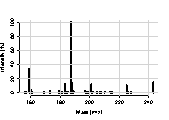
\includegraphics[width=3.1cm,height=1.65cm]{msms_spectrum.pdf}}; 
  \node (spectra) at (\xx+0.2*\xgap,\xy+2*\ygap) [database] { MS/MS Spectra };
  
  \node (feature) at (\xx+1*\xgap,\xy+2*\ygap) [database] { Molecular features };
  \node (retention) at (\xx+1.8*\xgap,\xy+2*\ygap) [database] { Retention time };

  \node (suptitle) at (\xx+1*\xgap,\xy+3.3*\ygap) [] {\color{blue} \Large Integration of MS/MS and retention order scores }; 
    
  \draw[->,line width=0.5mm] (spectra.south) to [out=270,in=90]
  (iokr.north) {};

  \draw[->,line width=0.5mm] (feature.south) to [out=270,in=90]
  node[above] {\footnotesize Fingerprints } (iokr.north) {};
  \draw[->,line width=0.5mm] (feature.south) to [out=270,in=90]
  node[above] {\footnotesize Fingerprints } (ranksvm.north) {};

  \draw[->,line width=0.5mm] (retention.south) to [out=270,in=90]
   (ranksvm.north) {};

  \draw[->,line width=0.5mm] (iokr.south) to [out=270,in=90]  (dynprog.north)  {};
  \draw[->,line width=0.5mm] (ranksvm.south) to [out=270,in=90]  (dynprog.north) {};



  \node[inner sep=0pt] (imfinger) at (\xx+0.95*\xgap,\xy+2.8*\ygap) {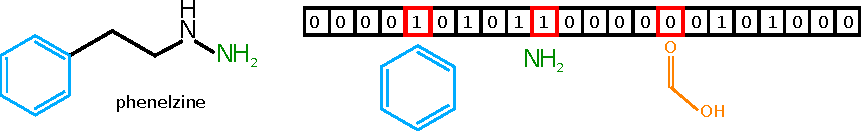
\includegraphics[width=4.2cm,height=0.7cm]{fingerprint_example.pdf}}; 

  \node[inner sep=0pt] (imretention) at (\xx+1.8*\xgap,\xy+2.8*\ygap) {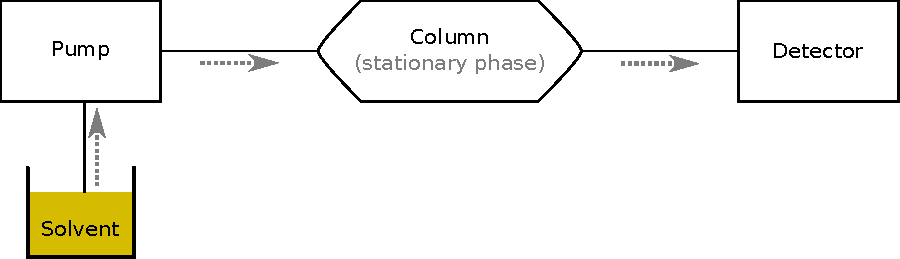
\includegraphics[width=4.2cm,height=1cm]{retention_time_example.pdf}}; 

  


\end{tikzpicture}


\end{document}
